\documentclass[12pt]{article}
\usepackage[margin=2.5cm]{geometry}
\usepackage{enumerate}
\usepackage{amsfonts}
\usepackage{amsmath}
\usepackage{fancyhdr}
\usepackage{amsmath}
\usepackage{amssymb}
\usepackage{amsthm}
\usepackage{mdframed}
\usepackage{graphicx}
\usepackage{subcaption}
\usepackage{adjustbox}
\usepackage{listings}
\usepackage{xcolor}
\usepackage{booktabs}
\usepackage[utf]{kotex}
\usepackage{hyperref}

\definecolor{codegreen}{rgb}{0,0.6,0}
\definecolor{codegray}{rgb}{0.5,0.5,0.5}
\definecolor{codepurple}{rgb}{0.58,0,0.82}
\definecolor{backcolour}{rgb}{0.95,0.95,0.92}

\lstdefinestyle{mystyle}{
    backgroundcolor=\color{backcolour},
    commentstyle=\color{codegreen},
    keywordstyle=\color{magenta},
    numberstyle=\tiny\color{codegray},
    stringstyle=\color{codepurple},
    basicstyle=\ttfamily\footnotesize,
    breakatwhitespace=false,
    breaklines=true,
    captionpos=b,
    keepspaces=true,
    numbers=left,
    numbersep=5pt,
    showspaces=false,
    showstringspaces=false,
    showtabs=false,
    tabsize=1
}

\lstset{style=mystyle}

\pagestyle{fancy}
\renewcommand{\headrulewidth}{0.4pt}
\lhead{Hyungmo Gu}
\rhead{CSC369 Week 3 Notes}

\begin{document}
\title{CSC369 Week 3 Notes}
\author{Hyungmo Gu}
\maketitle

\bigskip

\section{Synchronization}

\bigskip
\begin{itemize}
    \item Producer and Consumer Problem
    \begin{itemize}
        \item Is also known as \textbf{bound-and-buffer} problem
        \item Achieves synchronization
        \item Has two types of processes
        \begin{enumerate}[1.]
            \item \textbf{Producer}
            \begin{itemize}
                \item Produces data
                \item Puts data into buffer
            \end{itemize}
            \item \textbf{Consumer}
            \begin{itemize}
                \item Consumes data
                \item Removes data from buffer, one piece at a time
            \end{itemize}
        \end{enumerate}
        \item It's like kimchi factory, or delicious cookie factory :)

        \begin{center}
        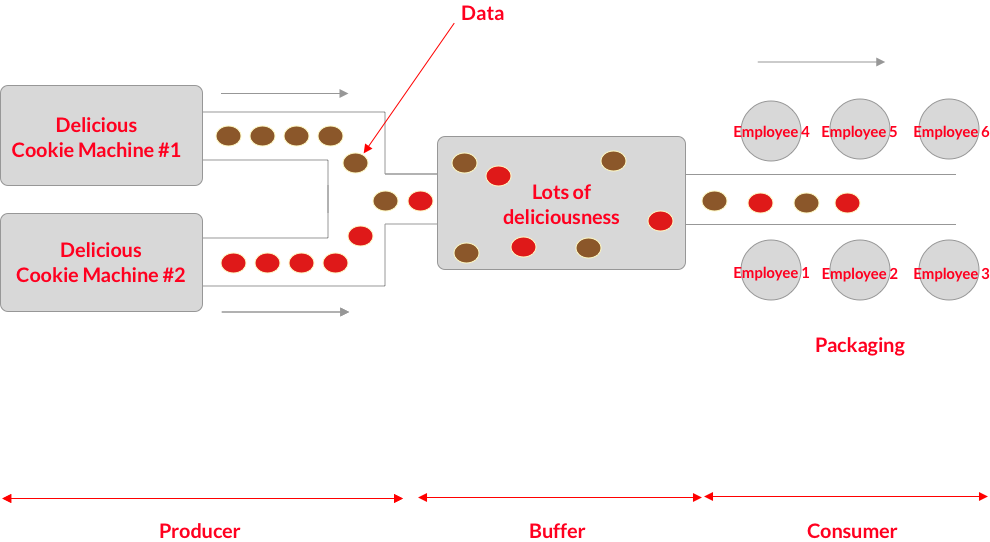
\includegraphics[width=\linewidth]{images/week_3_notes_1_1.png}
        \end{center}
    \end{itemize}

    \item Semaphore
    \begin{itemize}
        \item Developed by Dijkstra in 1962.
        \item is a signal
        \begin{itemize}
            \item Uses a non-negative integer variable that is shared between threads
            [\textit{Note: Need to come back later}]
            \item Has two ``\textbf{atomic}'' operations
            \begin{enumerate}[1.]
                \item \textbf{Wait} (Also called P, or decrement)
                \item \textbf{Signal} (Also called V, or increment)
            \end{enumerate}
        \end{itemize}
        \item Is easy to understand
        \item Is difficult to use
        \begin{itemize}
            \item One tiny mistake and everything comes to a halt
        \end{itemize}
    \end{itemize}

    \item Types of Semaphores
    \begin{enumerate}[1.]
        \item Counting Semaphore
        \begin{itemize}
            \item \textit{count = N} $\Rightarrow$ Max number of resources
            \item \textit{count} $\uparrow$ when resource added
            \item \textit{count} $\downarrow$ when resource used
            \item \textit{count = 0} $\Rightarrow$ No resources available $\Rightarrow$ \textbf{Wait} until \textit{count \textgreater 0}
        \end{itemize}

        \begin{center}
        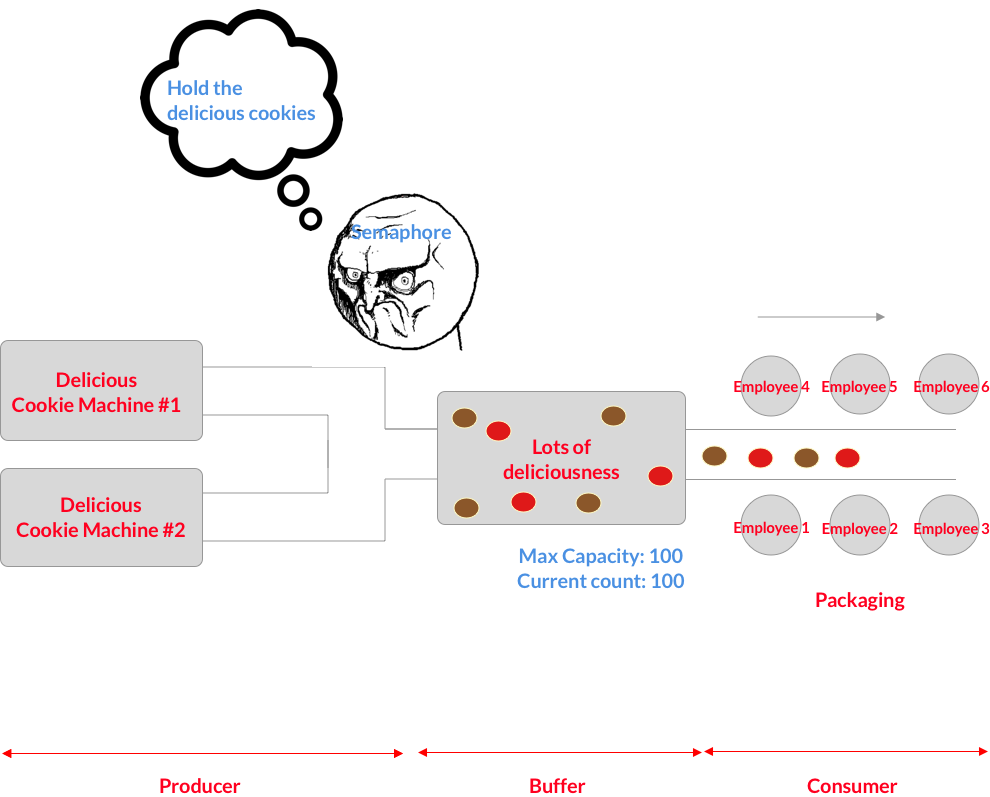
\includegraphics[width=0.8\linewidth]{images/week_3_notes_1_3.png}
        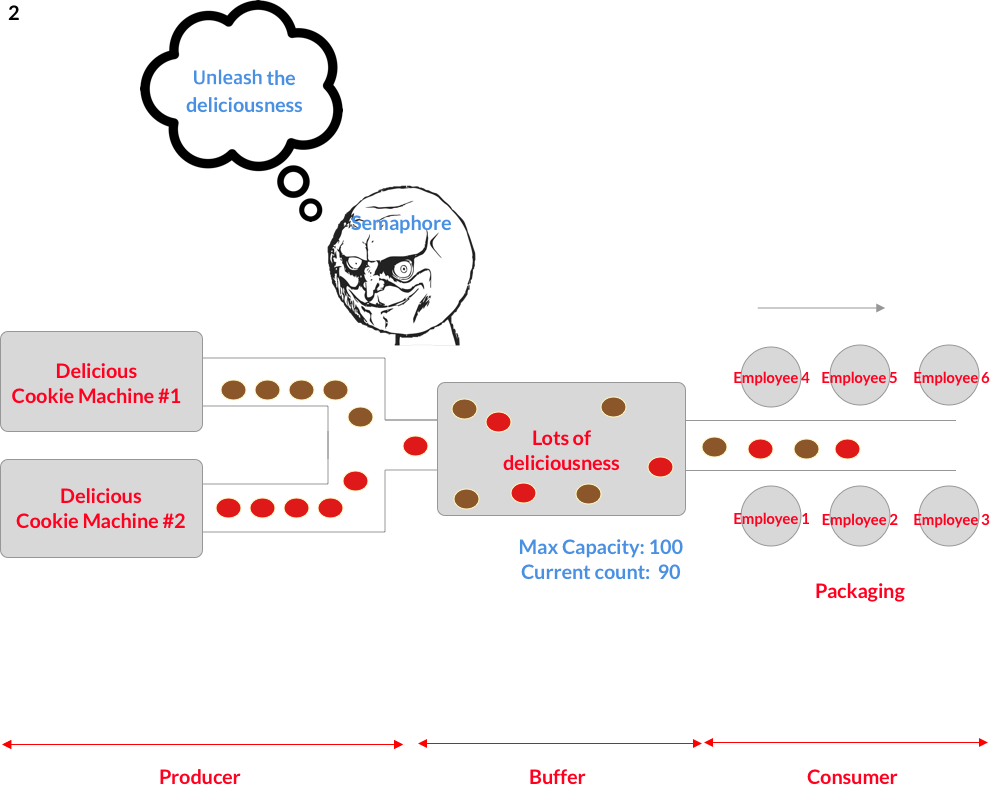
\includegraphics[width=0.8\linewidth]{images/week_3_notes_1_4.png}
        \end{center}

        \item Binary Semaphore
        \begin{itemize}
            \item \textit{count = 1} $\Rightarrow$ Unlocked / Available
            \begin{itemize}
                \item A thread can go in
            \end{itemize}
            \item \textit{count = 0} $\Rightarrow$ Locked / Unavailable $\Rightarrow$ \textbf{Wait} until
            \textit{count \textgreater 0}
            \begin{itemize}
                \item Other threads must wait
            \end{itemize}
            \item It's like the security at airport, or the portable bathroom from
            week 1 notes
        \end{itemize}

        \begin{center}
        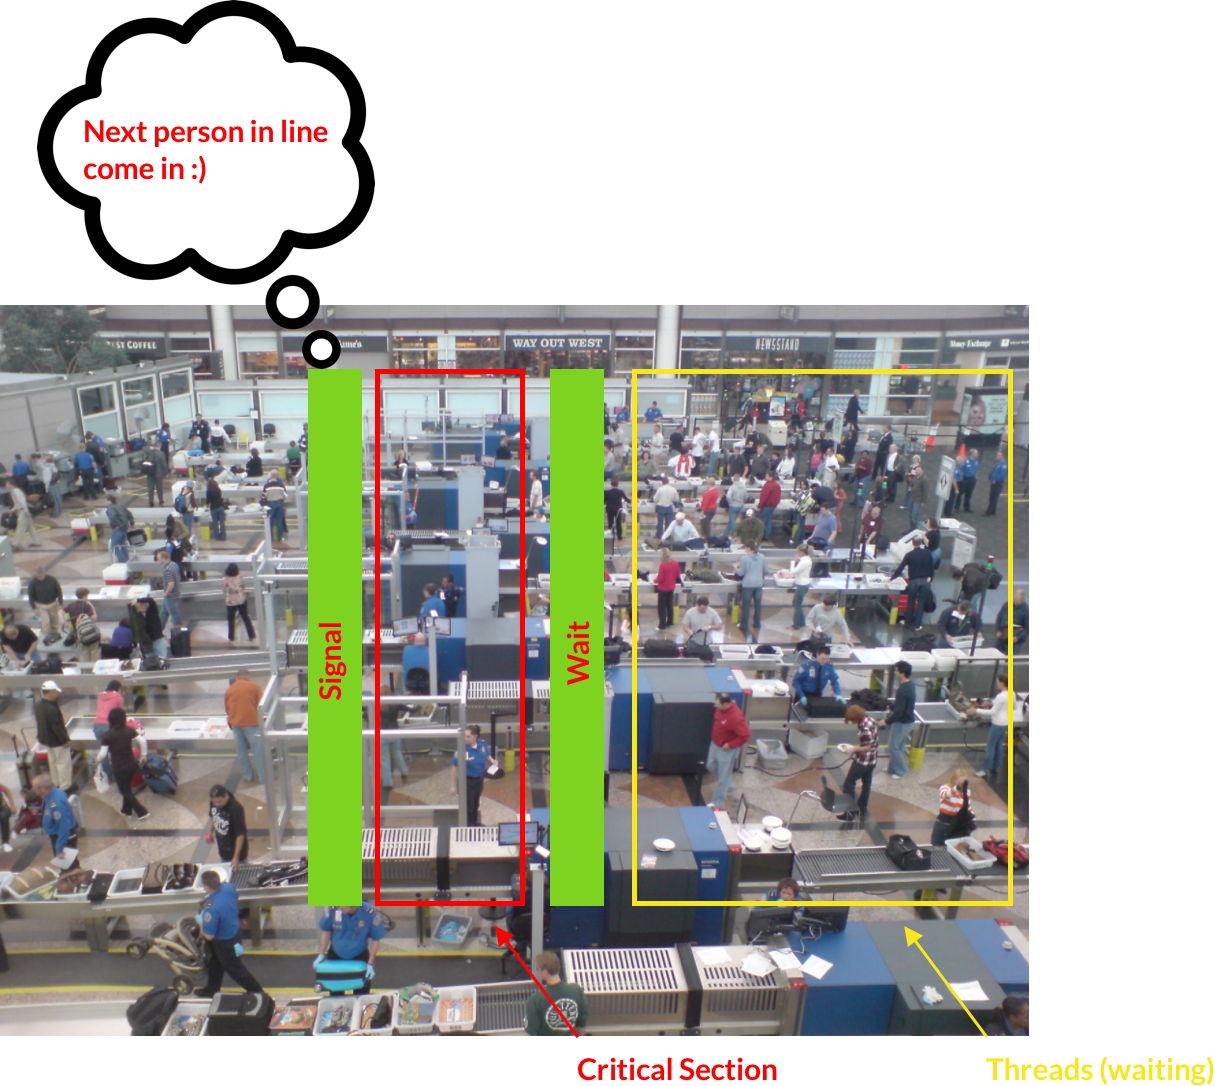
\includegraphics[width=0.8\linewidth]{images/week_3_notes_1_5.png}
        \end{center}
    \end{enumerate}
    % \item Using Binary Semaphores
    % \item Atomicity of wait() and signal()
    % \item Read-write problem
    % \item Reader's operation
    % \item Writer's operation
    % \item Reader's and Writer's Operation
    % \item Notes on Readers/Writers
    \item Monitors
    \begin{itemize}
        \item Is solution to semaphore
        \begin{itemize}
            \item Is easier to implement
            \item Creates less bugs
        \end{itemize}
        \item Still not a good solution
        \begin{itemize}
            \item Usable only in few programming languages
            \begin{itemize}
                \item C not supported
                \item Java supported
            \end{itemize}
            \item Is designed for single or multiple CPUS with access to a common
            memory
            \item Not designed for the age of internet
            \begin{itemize}
                \item Fails with distributed system with each having private memory
                connected via internet
                \item Can't exchange information between machines
            \end{itemize}
        \end{itemize}
    \end{itemize}
\end{itemize}

\bigskip

\section{Intro to Scheduling}

\bigskip

\begin{itemize}
    % \item State Queues
    % \item Proccessor Scheduling
    % \item What Happens on Dispatch / Context Switch
    % \item Process Life Cycle
    \item What is Proceess Scheduling
    \begin{itemize}
        \item Is a process at which allows one process to use the CPU while
        another is on hold, to make full use of CPU $^{[1]}$
        \item This is key to multi-programming
    \end{itemize}

    \bigskip

    \underline{\textbf{References}}

    \bigskip

    \begin{enumerate}[1)]
        \item Study Tonight: What is CPU Scheduling?, \href{https://www.studytonight.com/operating-system/cpu-scheduling}{link}
        \item University of Illinois: CPU Scheduling, \href{https://www.cs.uic.edu/~jbell/CourseNotes/OperatingSystems/6_CPU_Scheduling.html}{link}
    \end{enumerate}

    % \item When to Schedule
    % \item Scheduling Goals
    \item Types of Scheduling
    \begin{itemize}
        \item Non-preemtive Scheduling
        \begin{itemize}
            \item Once the the CPU has been allocated to a process, the CPU
            keeps the process until it releases either by terminating or by switching
            to the waiting state $^{[1]}$

            \begin{center}
            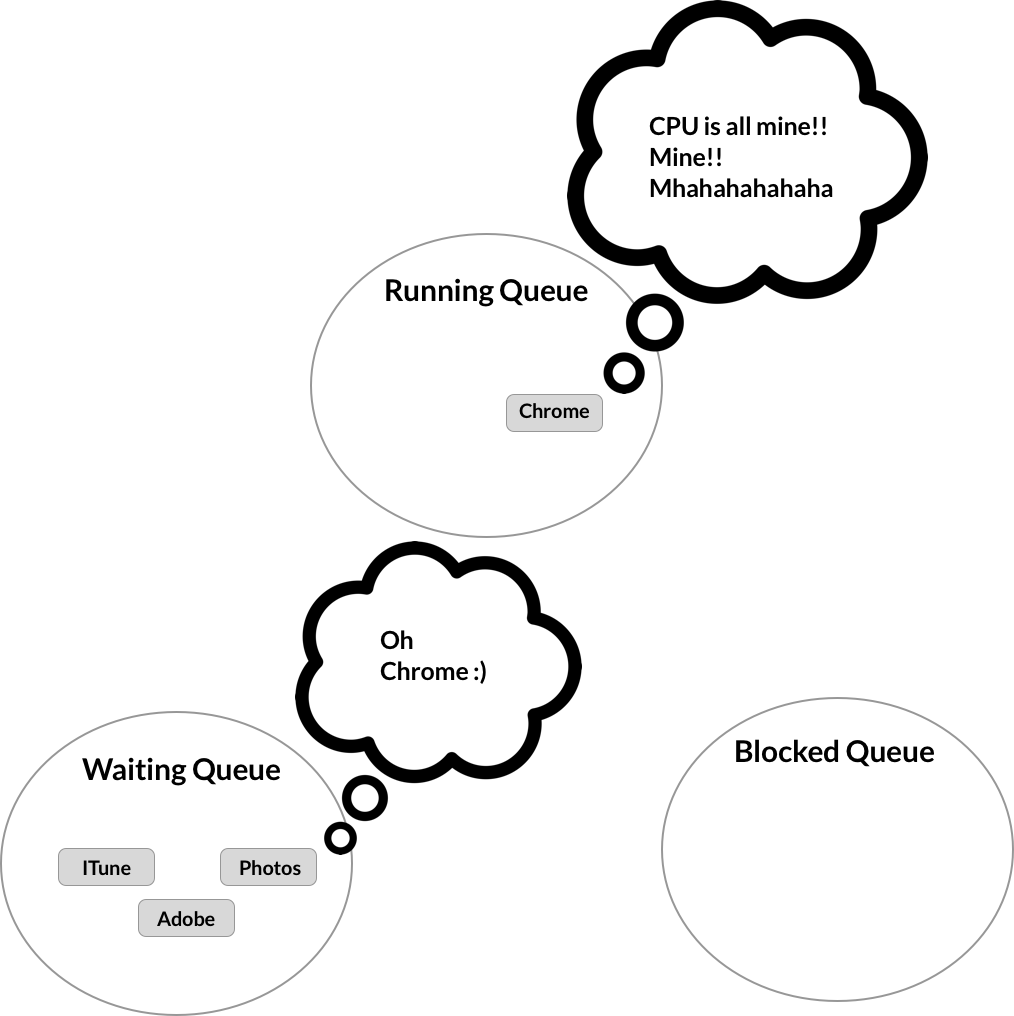
\includegraphics[width=0.8\linewidth]{images/week_3_notes_2_1.png}
            \end{center}

            \item e.g Windows 3.1
            \item Suitable for batch scheduling
        \end{itemize}
        \item Preemptive Scheduling
        \begin{itemize}
            \item Usually assigns tasks with prioirities $^{[1]}$
            \item Can interrupt for higher priority task $^{[1]}$
            \item Resumes existing task once priority task completes execution $^{[1]}$
            \item Needed in interactive or real time systems
            \item Feels like juggling
        \end{itemize}
    \end{itemize}

    \bigskip

    \underline{\textbf{References}}

    \bigskip

    \begin{enumerate}[1)]
        \item Study Tonight: What is CPU Scheduling?, \href{https://www.studytonight.com/operating-system/cpu-scheduling}{link}
    \end{enumerate}
\end{itemize}

\end{document}